\documentclass[a4paper]{article}
\usepackage[top=2cm, bottom=2cm, outer=0cm, inner=0cm]{geometry}
\usepackage[pages=some]{background}
\backgroundsetup{scale=1, color=black, opacity=1, angle=0, contents={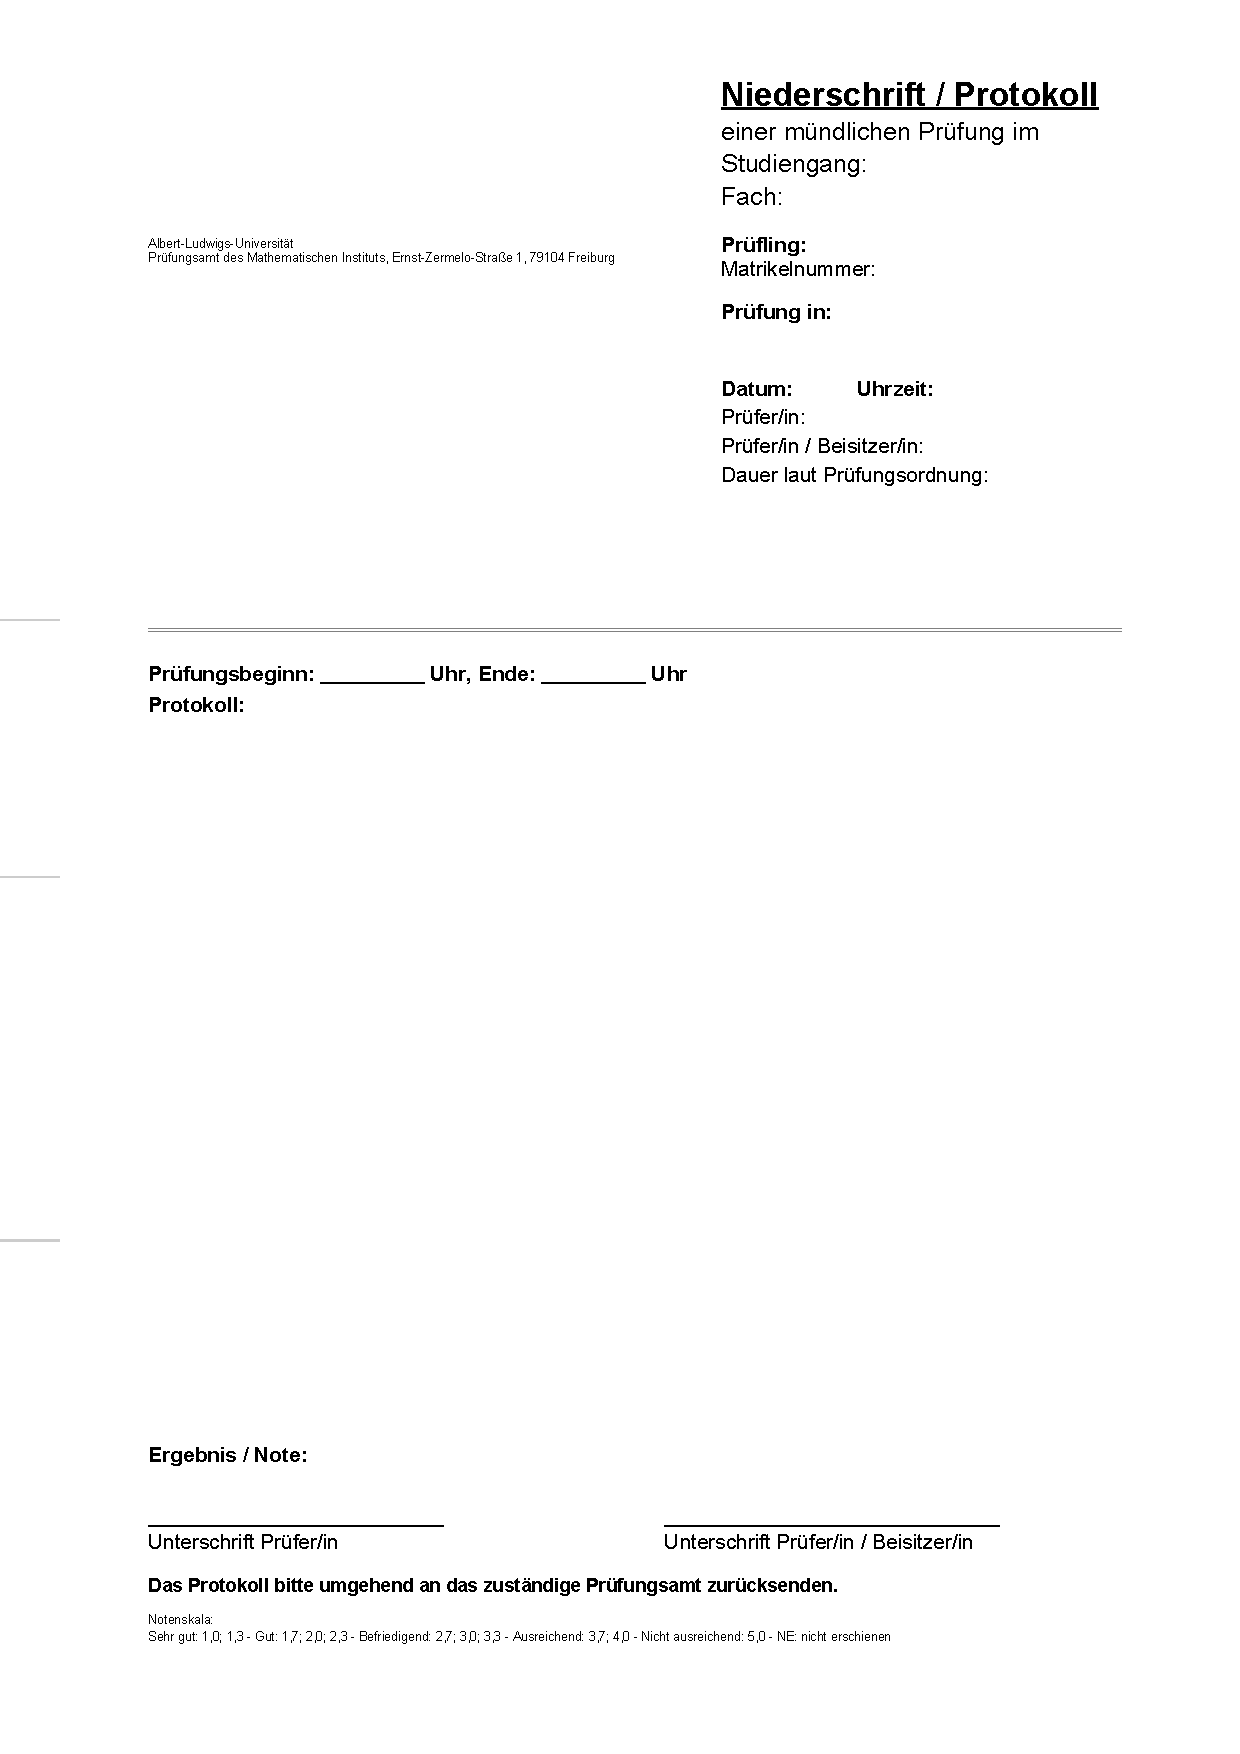
\includegraphics[width=\paperwidth,height=\paperheight]{../Niederschrift_Hintergrund.pdf}}}

\usepackage[overlay,absolute]{textpos}
\newcommand\PlaceText[3]{%
\begin{textblock*}{10in}(#1,#2)  %% change width of box from 10in as you wish
#3
\end{textblock*}
}%
\textblockorigin{-5mm}{0mm}   %% Default origin top left corner and it can be changed in this line

\begin{document}
\thispagestyle{empty}
 \BgThispage

 \PlaceText{150mm}{27mm}{\VAR{prüfung['Studiengang']}}
 \PlaceText{150mm}{31mm}{Mathematik}
 \PlaceText{150mm}{40mm}{\VAR{prüfung['Vorname']} \VAR{prüfung['Nachname']}}
 \PlaceText{150mm}{44mm}{\VAR{prüfung['Matrikelnummer']}}
 \PlaceText{150mm}{51.5mm}{\VAR{prüfung['Fach']}}
 \PlaceText{122mm}{60mm}{\VAR{prüfung['Datum']}}
 \PlaceText{145mm}{60mm}{\VAR{prüfung['Uhrzeit']}}
 \PlaceText{140mm}{69.5mm}{\VAR{prüfung['Prüfer_Vorname']} \VAR{prüfung['Prüfer_Nachname']}}
% \PlaceText{158mm}{74mm}{\VAR{prüfung['beisitzer']}}
 \PlaceText{168mm}{79mm}{30 Minuten}
% \PlaceText{122mm}{85mm}{Prüfungsnummer: \VAR{prüfung['pr_nummer']}}
 
 \end{document}
